\documentclass{beamer}
\usetheme{Madrid}

\usepackage{amsmath, amssymb, amsthm}
\usepackage{graphicx}
\usepackage{gensymb}
\usepackage[utf8]{inputenc}
\usepackage{hyperref}
\usepackage{tikz}


\title{2.6.12 }
\author{AI25BTECH11006 - Nikhila}
\date{31-08-2025}

\begin{document}

\frame{\titlepage}

% Question frame
\begin{frame}
\frametitle{Question}
Find the sine of the angle between the vectors $\vec{a} = 3\hat{i} + \hat{j} + 2\hat{k}$ and $\vec{b} = 2\hat{i} + -2\hat{j} + 4\hat{k}$.\\
 \end{frame}




% Solution steps
\begin{frame}
\frametitle{Solution}
The given vectors are $\vec{a}\begin{pmatrix}3 \\ 1 \\ 2\end{pmatrix} $ and $  \vec{b}\begin{pmatrix}2 \\ -2 \\ 4\end{pmatrix}$ \\ 
 We know that 
\begin{align}
|\vec{a}\times\vec{b}| = |\vec{a}| \hspace{0.3em} |\vec{b}| \sin\theta \\
\sin\theta = \frac{|\vec{a}\times\vec{b}|}{|\vec{a}||\vec{b}|}.
\end{align}

\begin{align}
\vec{a} \times \vec{b} = 
\begin{pmatrix}
 3 \\ 1 \\ 2  
\end{pmatrix} \times \begin{pmatrix}
 2 \\ -2 \\ 4  
\end{pmatrix} = 8 \begin{pmatrix} 1 \\ -1 \\ -1 \end{pmatrix}
\end{align}
\begin{align}    
\lVert \vec{a}\times\vec{b} \rVert  =  8\sqrt{3}
\end{align}

\end{frame}


\begin{frame}
\frametitle{Solution}

\begin{align}
|\vec{a}| &= \sqrt{(3)^2 + (1)^2 + (2)^2} = \sqrt{14}, \\
|\vec{b}| &= \sqrt{(2)^2 + (-2)^2 + (4)^2} = \sqrt{24}.
\end{align}

\begin{align}
\sin\theta &= \frac{|\vec{a}\times \vec{b}|}{|\vec{a}||\vec{b}|} \\
&= \frac{8\sqrt{3}}{\sqrt{14}\cdot \sqrt{24}} \\
&= \frac{2}{\sqrt{7}}.
\end{align}

 \end{frame}


% Graphical representation
\begin{frame}
\frametitle{Graphical Representation}
\begin{center}
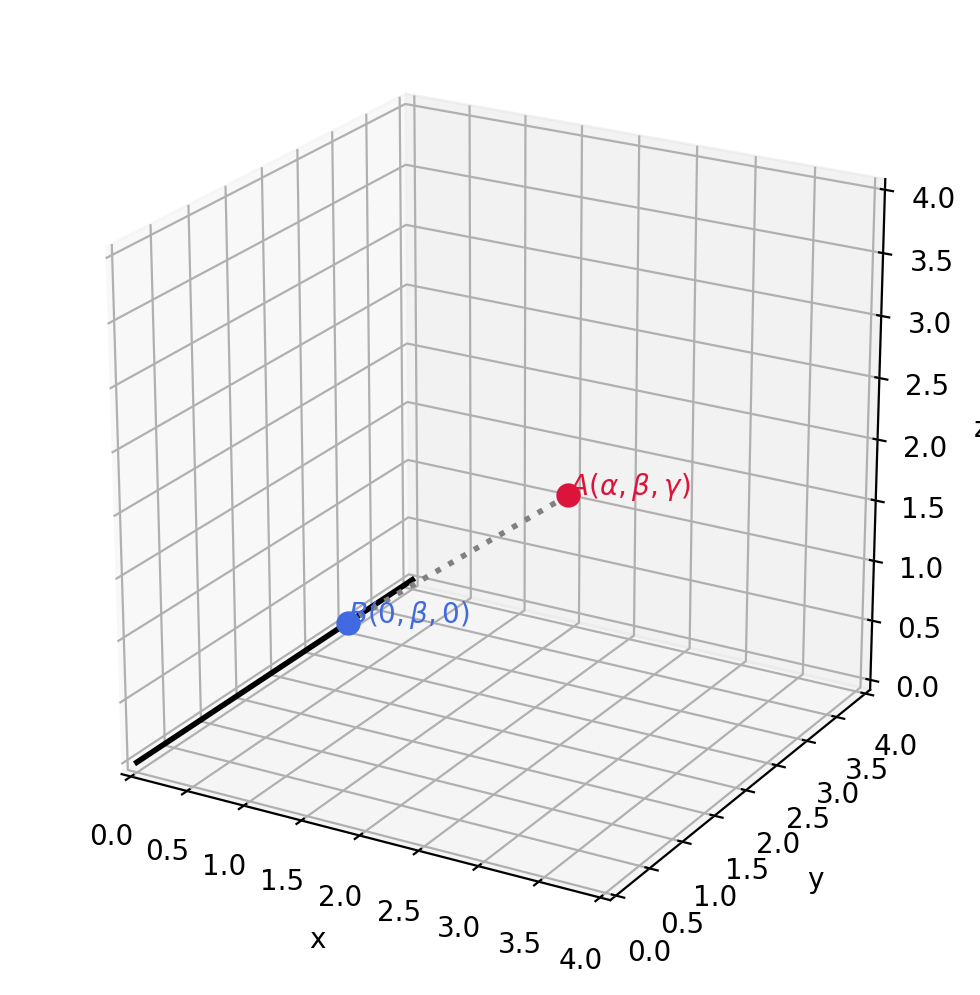
\includegraphics[width=0.8\linewidth]{fig1.png}
\end{center}
\end{frame}

\end{document}
